\documentclass[11pt,a4paper,twoside]{article}
\usepackage[top=2cm, bottom=2cm, left=2cm, right=2cm]{geometry}  % nustatomos paraštės
\usepackage[T1]{fontenc}		% LT raidėms su Helvetica
\usepackage[utf8]{inputenc}		% šriftams
%\def\LTfontencoding{L7x}		% LT raidėms su Times New Roman
%\usepackage[L7x]{fontenc}
\usepackage[lithuanian]{babel}	% sulietuvinimas
\usepackage{graphicx}			% paveikslams
\usepackage{caption}			% paveikslu aprašams
\usepackage{subcaption}			% paveikslu aprašams
\usepackage{amsmath}			% formulėms
\usepackage{amsthm}				% sudėtingoms formulėms
\usepackage{amsfonts}			% matematiniams šriftams
\usepackage{pifont}				% šriftams
\usepackage{gensymb}			% matematiniams simboliams
\usepackage{enumerate}			% numeracijai
\usepackage{float}				% paveikslų ir lentelių pozicionavimui
\usepackage[version=3]{mhchem}	% cheminėms formulėms
\usepackage{multirow}			% lentelėms
\usepackage{lmodern}	    	% kitiem šriftam
\usepackage{afterpage}			% formatavimui
\usepackage{setspace}			% tarpui tarp eilučių
\usepackage{hyperref}			% komanda sukuria nuorodas
\hypersetup{					% nuorodos nespalvinamos
	colorlinks,%
	citecolor=black,%
	filecolor=black,%
	linkcolor=black,%
	urlcolor=black
}

\usepackage[scaled]{helvet}			% Helvetica šrifto paketas
\renewcommand{\familydefault}{\sfdefault} % pagrindinio šrifot pakeitimas į Sans, šiuo atveju Helvetica

\begin{document}
\sloppy					% neleidžia tekstui išlįsti į paraštes


\title{$Z^0$ decay into $\mu^{+}$ and $\mu^{-}$}
\author{Nikolajus Elkana Eimutis \\ Taikomoji fizika, Fizikos fakultetas, Vilniaus Universitetas}
\maketitle

\onehalfspace

\paragraph*{Goal:}
Using LHCb open data measure Z boson mass and other important variables (observables?).


\section{Milestones}

\begin{enumerate}
        \item Data is downloaded and ready for local analysis.
        
        \item Theoretical understanding of how LHCb gathers its data is developed.
        
        \item Theoretical understanding of how two muons arise from two protons is developed.

        \item Pratical skill to write root macros is learned.

        \item The data is filtered in such a manner that there is only one evident peak in the Z boson mass graph.

        \item A boson mass graph is drawn, the data is fitted against appropriate theoretical function.
\end{enumerate}
	
% \thispagestyle{empty}			%opcija nenumeruoti pirmojo psl.
\newpage


\section{Theory}
    \begin{enumerate}
        \item Feynman diagrams

        They are figurative depictions of contributions from interactions between particles, which are described by quantum field theory\cite{Jende_Kobel_Pospiech_Bilow_Pedersen_Ould-Saada_Gramstad}.

        \begin{figure}[H]
            \centering

            \subfloat[\centering muon-antimuon anihilation \cite{Jende_Kobel_Pospiech_Bilow_Pedersen_Ould-Saada_Gramstad}.]{{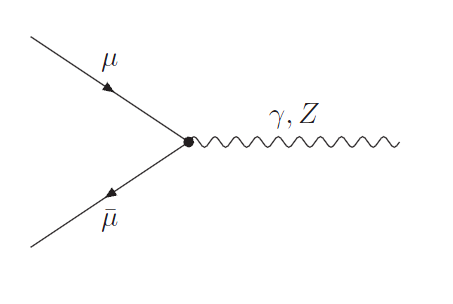
\includegraphics[width=0.5\textwidth]{visuals/002-MuonAntimuonAnihilation.png} }}%
            \subfloat[\centering $Z^0$ decay into muon-antimuon pair \cite{Jende_Kobel_Pospiech_Bilow_Pedersen_Ould-Saada_Gramstad}.]{{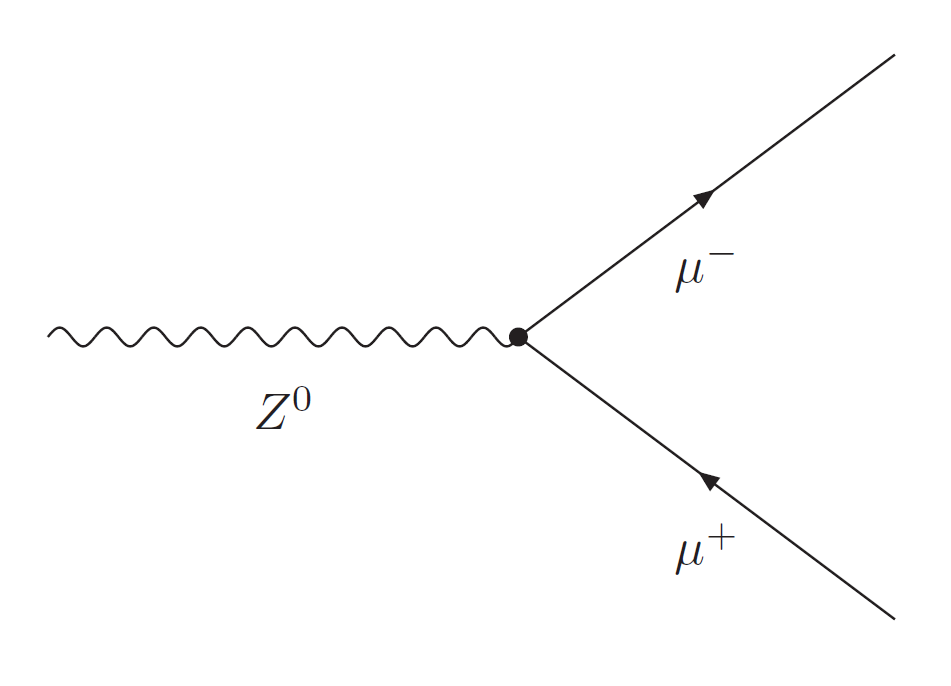
\includegraphics[width=0.5\textwidth]{visuals/001-Z_MyonAntimyon.png} }}%
            
        
        
            \caption{Feynman diagrams for the processes with Z boson and muon-antimuon pair.}
            \label{fig:001-Z_MyonAntimyon}
        \end{figure}


        \textbf{[TODO: maybe add more complicated diagrams, if something is relevant]}

        
        \textbf{[TODO: maybe address the Drell-Yan process here]}


        \item Processes mimicking Z boson signal

        \textbf{[TODO: answer]}

        
        \item Main graphs and charts drawn when analysing Z boson decay into two muons. What properties are usually analysed?


        Most accurately known parameters (at least back in 1999) are $G_{\mu}$, $\bar{\alpha}$, $m_Z$ \cite{novikov1999theory};


        Possibly useful, since the paper is very similar to this one: muon, Z-boson momentum, pseudorapidity \cite{khodaverdian2019accuracy};

        \textbf{[TODO: add more descriptions and explanations here]}


        \item Theoretical calculation of Z boson mass from two muons.

        Born model[\textbf{[TODO: ?]}]


        \textbf{[TODO: answer]}

        \item LHCb detector structure, trigger, reconstruction, data validity and error.

        \textbf{[TODO: answer]}

        \item Data types used in LHCb.

        \textbf{[TODO: answer]}
        
    \end{enumerate}


\section{Results}
    
\singlespacing
	
	%\phantomsection
	
\bibliographystyle{VUstyle}
\bibliography{mybib}
	
\end{document}
